\subsection{Подзапросы}
\begin{frame}
	\tableofcontents[currentsection,currentsubsection]
\end{frame}

\begin{frame}{Подзапросы-1}
	\begin{enumerate}
		\item
			\begin{itemize}
				\item Задача: хотим для города найти население страны, в которой он расположен.
				\item В таблице городов есть только код страны, без населения.
				\item Можно сделать подзапрос в условии \t{WHERE}.
			\end{itemize}
		\item
			\begin{itemize}
				\item Задача: рассмотрим в каждый год самую грамотную страну и её уровень грамотности, хотим найти средний уровень по годам.
				\item Надо две агрегатных функции: сначала группируем по годам (чтобы найти победителя), а потом берём среднее.
				\item Можно сделать подзапрос в \t{FROM} (ведь результат SELECT "--- тоже таблица, которую можно назвать).
			\end{itemize}
	\end{enumerate}
\end{frame}

\begin{frame}{Подзапросы-2}
	\begin{itemize}
		\item Задача: хотим вывести информацию по странам плюс население самого большого города.
		\item Эта информация лежит в двух разных таблицах.
		\item SQL позволяет делать \t{SELECT FROM} сразу из нескольких таблиц (получается декартово произведение).
		\item Можно взять декартово произведение городов и стран, оставить только соответствующие, а по оставшимся взять агрегирующую функцию.
		\item Если имена колонок в разных таблицах совпадают, надо явно указывать, к какой мы обращаемся.
		\item Вообще лучше всегда явно указывать, из какой таблицы мы берём колонку, если таблиц несколько.
	\end{itemize}
	Такого сорта выборки происходят очень часто, в реляционной алгебре они зовутся <<соединениями>> (join).
\end{frame}

\subsection{Соединения}
\begin{frame}
	\tableofcontents[currentsection,currentsubsection]
\end{frame}

\begin{frame}{Соединения}
	\begin{itemize}
		\item Можно считать синтаксическим сахаром для взятия подмножества декартова произведения.
		\item Лучше отражает суть происходящего и проще читается.
		\item После \t{ON} может быть произвольное условие (это круче, чем в реляционной алгебре).
		\item Обычно там ставят условие <<номер страны в первой таблице равен номеру страны во второй таблице>>.
	\end{itemize}
\end{frame}

\begin{frame}[fragile]{Соединения "--- картинка}
	\svgimg{join-01}
\end{frame}

\begin{frame}{Ключи и соединения-1}
	\begin{itemize}
		\item Обычно сущностей в базе много и они как-то связны отношениями (<<каждый город лежит ровно в одной стране>>).
		\item Не хочется дублировать информацию в разных таблицах (место занимает, изменять сложно).
		\item Поэтому информация о стране/городе отдельно.
		\item А запрос <<получи объект по вот этому отношению>> возникает.
		\item
			Так как свойства объектов часто меняются, то обычно каждому объекту выдают \textit{первичный ключ},
			по которому его можно опознать.
			Обычно это просто какое-то число (возможно, с автоинкрементом).
	\end{itemize}
\end{frame}

\begin{frame}{Ключи и соединения-2}
	\begin{itemize}
		\item Тогда связи вроде <<в какой стране лежит город>> "--- это просто столбец <<номер страны>> в таблице с городом.
		\item Такой столбец называют \textit{внешним ключом}.
		\item Это даже можно отразить в структуре таблицы (\t{REFERENCES}).
		\item И ещё можно указать, что делать при удалении того объекта, куда мы ссылаемся (\t{ON DELETE CASCADE}).
	\end{itemize}
\end{frame}

\begin{frame}{Упражнения}
	\begin{enumerate}
		\item Вывести для каждой страны её имя и максимальный уровень её грамотности за все года.
		\item Вывести для каждой страны её имя и номер города-столицы (см. таблицу \t{Capital}).
		\item Вывести для каждой страны её имя и название города-столицы (потребуется два \t{JOIN}).
	\end{enumerate}
\end{frame}

\begin{frame}{Соединения, NULL, отсутствие значений}
	\begin{enumerate}
		\item Посчитаем количество стран (239).
		\item Теперь для каждой страны посчитаем количество городов.
		\item Теперь посмотрим, сколько строк получили в результате "--- 232.
	\end{enumerate}
	\begin{itemize}
		\item А всё потому что есть страны, в которых городов нет "--- про них в таблице \t{City} просто нет информации.
		\item И соединение не поможет "--- страна без городов отфильтруется.
		\item Но есть \t{LEFT (OUTER) JOIN} "--- он обязуется добавить в соединение все строчки из <<левой>> таблицы
			(а если не нашлось соответствующих строк, то поля второй в строчке соединения будут \t{NULL}).
		\item С ним надо быть осторожным "--- потому что теперь в строчках соединения могут оказаться \t{NULL},
			которые, скорее всего, не надо учитывать (\t{COUNT(*)}, например, их учтёт).
		\item Ещё бывают аналогичные \t{RIGHT JOIN} и \t{FULL JOIN} (SQLite их не поддерживает).
	\end{itemize}
\end{frame}

\begin{frame}[fragile]{Соединения "--- картинка}
	\svgimg{join-02}
\end{frame}

\begin{frame}{Классическая шутка}
	\begin{center}
		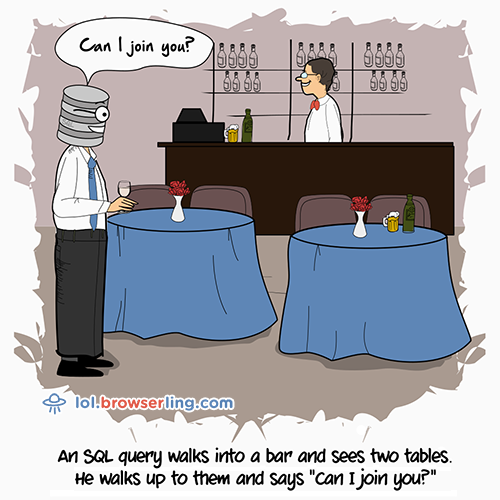
\includegraphics[scale=0.4]{join-two-tables.png}

		\href{https://comic.browserling.com/23}{comic.browserling.com/23}
	\end{center}
\end{frame}
